\documentclass[twoside]{book}

% Packages required by doxygen
\usepackage{calc}
\usepackage{doxygen}
\usepackage{graphicx}
\usepackage[utf8]{inputenc}
\usepackage{makeidx}
\usepackage{multicol}
\usepackage{multirow}
\usepackage{textcomp}
\usepackage[table]{xcolor}

% Font selection
\usepackage[T1]{fontenc}
\usepackage{mathptmx}
\usepackage[scaled=.90]{helvet}
\usepackage{courier}
\usepackage{amssymb}
\usepackage{sectsty}
\renewcommand{\familydefault}{\sfdefault}
\allsectionsfont{%
  \fontseries{bc}\selectfont%
  \color{darkgray}%
}
\renewcommand{\DoxyLabelFont}{%
  \fontseries{bc}\selectfont%
  \color{darkgray}%
}

% Page & text layout
\usepackage{geometry}
\geometry{%
  a4paper,%
  top=2.5cm,%
  bottom=2.5cm,%
  left=2.5cm,%
  right=2.5cm%
}
\tolerance=750
\hfuzz=15pt
\hbadness=750
\setlength{\emergencystretch}{15pt}
\setlength{\parindent}{0cm}
\setlength{\parskip}{0.2cm}
\makeatletter
\renewcommand{\paragraph}{%
  \@startsection{paragraph}{4}{0ex}{-1.0ex}{1.0ex}{%
    \normalfont\normalsize\bfseries\SS@parafont%
  }%
}
\renewcommand{\subparagraph}{%
  \@startsection{subparagraph}{5}{0ex}{-1.0ex}{1.0ex}{%
    \normalfont\normalsize\bfseries\SS@subparafont%
  }%
}
\makeatother

% Headers & footers
\usepackage{fancyhdr}
\pagestyle{fancyplain}
\fancyhead[LE]{\fancyplain{}{\bfseries\thepage}}
\fancyhead[CE]{\fancyplain{}{}}
\fancyhead[RE]{\fancyplain{}{\bfseries\leftmark}}
\fancyhead[LO]{\fancyplain{}{\bfseries\rightmark}}
\fancyhead[CO]{\fancyplain{}{}}
\fancyhead[RO]{\fancyplain{}{\bfseries\thepage}}
\fancyfoot[LE]{\fancyplain{}{}}
\fancyfoot[CE]{\fancyplain{}{}}
\fancyfoot[RE]{\fancyplain{}{\bfseries\scriptsize Generated on Mon Jul 8 2013 04:47:09 for Sudoku by Doxygen }}
\fancyfoot[LO]{\fancyplain{}{\bfseries\scriptsize Generated on Mon Jul 8 2013 04:47:09 for Sudoku by Doxygen }}
\fancyfoot[CO]{\fancyplain{}{}}
\fancyfoot[RO]{\fancyplain{}{}}
\renewcommand{\footrulewidth}{0.4pt}
\renewcommand{\chaptermark}[1]{%
  \markboth{#1}{}%
}
\renewcommand{\sectionmark}[1]{%
  \markright{\thesection\ #1}%
}

% Indices & bibliography
\usepackage{natbib}
\usepackage[titles]{tocloft}
\setcounter{tocdepth}{3}
\setcounter{secnumdepth}{5}
\makeindex

% Hyperlinks (required, but should be loaded last)
\usepackage{ifpdf}
\ifpdf
  \usepackage[pdftex,pagebackref=true]{hyperref}
\else
  \usepackage[ps2pdf,pagebackref=true]{hyperref}
\fi
\hypersetup{%
  colorlinks=true,%
  linkcolor=blue,%
  citecolor=blue,%
  unicode%
}

% Custom commands
\newcommand{\clearemptydoublepage}{%
  \newpage{\pagestyle{empty}\cleardoublepage}%
}


%===== C O N T E N T S =====

\begin{document}

% Titlepage & ToC
\hypersetup{pageanchor=false}
\pagenumbering{roman}
\begin{titlepage}
\vspace*{7cm}
\begin{center}%
{\Large Sudoku \\[1ex]\large 1.\-2 }\\
\vspace*{1cm}
{\large Generated by Doxygen 1.8.4}\\
\vspace*{0.5cm}
{\small Mon Jul 8 2013 04:47:09}\\
\end{center}
\end{titlepage}
\clearemptydoublepage
\tableofcontents
\clearemptydoublepage
\pagenumbering{arabic}
\hypersetup{pageanchor=true}

%--- Begin generated contents ---
\chapter{Hierarchical Index}
\section{Class Hierarchy}
This inheritance list is sorted roughly, but not completely, alphabetically\-:\begin{DoxyCompactList}
\item \contentsline{section}{Dimensiones}{\pageref{class_dimensiones}}{}
\item \contentsline{section}{Generador}{\pageref{class_generador}}{}
\item Q\-Main\-Window\begin{DoxyCompactList}
\item \contentsline{section}{Main\-Window}{\pageref{class_main_window}}{}
\end{DoxyCompactList}
\item Q\-Widget\begin{DoxyCompactList}
\item \contentsline{section}{Numero}{\pageref{class_numero}}{}
\end{DoxyCompactList}
\end{DoxyCompactList}

\chapter{Class Index}
\section{Class List}
Here are the classes, structs, unions and interfaces with brief descriptions\-:\begin{DoxyCompactList}
\item\contentsline{section}{\hyperlink{class_dimensiones}{Dimensiones} }{\pageref{class_dimensiones}}{}
\item\contentsline{section}{\hyperlink{class_generador}{Generador} }{\pageref{class_generador}}{}
\item\contentsline{section}{\hyperlink{class_main_window}{Main\-Window} }{\pageref{class_main_window}}{}
\item\contentsline{section}{\hyperlink{class_numero}{Numero} }{\pageref{class_numero}}{}
\end{DoxyCompactList}

\chapter{File Index}
\section{File List}
Here is a list of all documented files with brief descriptions\-:\begin{DoxyCompactList}
\item\contentsline{section}{C\-:/\-Users/user/\-Documents/\-Git\-Hub/\-Sudoku/\-Sudoku/{\bfseries Dimensiones.\-h} }{\pageref{_dimensiones_8h}}{}
\item\contentsline{section}{C\-:/\-Users/user/\-Documents/\-Git\-Hub/\-Sudoku/\-Sudoku/\hyperlink{generador_8h}{generador.\-h} \\*Este archivo contiene la interfaz del generador de Sudokus }{\pageref{generador_8h}}{}
\item\contentsline{section}{C\-:/\-Users/user/\-Documents/\-Git\-Hub/\-Sudoku/\-Sudoku/\hyperlink{mainwindow_8h}{mainwindow.\-h} \\*Este archivo contiene la interfaz de la ventana principal }{\pageref{mainwindow_8h}}{}
\item\contentsline{section}{C\-:/\-Users/user/\-Documents/\-Git\-Hub/\-Sudoku/\-Sudoku/{\bfseries Mejores\-Puntajes.\-h} }{\pageref{_mejores_puntajes_8h}}{}
\item\contentsline{section}{C\-:/\-Users/user/\-Documents/\-Git\-Hub/\-Sudoku/\-Sudoku/{\bfseries mejorestiempos.\-h} }{\pageref{mejorestiempos_8h}}{}
\item\contentsline{section}{C\-:/\-Users/user/\-Documents/\-Git\-Hub/\-Sudoku/\-Sudoku/\hyperlink{numero_8h}{numero.\-h} \\*Este archivo contiene la interfaz de la clase \hyperlink{class_numero}{Numero} }{\pageref{numero_8h}}{}
\item\contentsline{section}{C\-:/\-Users/user/\-Documents/\-Git\-Hub/\-Sudoku/\-Sudoku/\hyperlink{_posicion_8h}{Posicion.\-h} \\*Este archivo contiene la interfaz de la clase \hyperlink{class_posicion}{Posicion} }{\pageref{_posicion_8h}}{}
\item\contentsline{section}{C\-:/\-Users/user/\-Documents/\-Git\-Hub/\-Sudoku/\-Sudoku/\hyperlink{puntaje_8h}{puntaje.\-h} \\*Este archivo contiene la interfaz de la clase \hyperlink{class_puntaje}{Puntaje} }{\pageref{puntaje_8h}}{}
\end{DoxyCompactList}

\chapter{Class Documentation}
\hypertarget{class_dimensiones}{\section{Dimensiones Class Reference}
\label{class_dimensiones}\index{Dimensiones@{Dimensiones}}
}
\subsection*{Static Public Attributes}
\begin{DoxyCompactItemize}
\item 
\hypertarget{class_dimensiones_a2fb9391d1230b6cc7a2a4008e74bcddc}{static const int {\bfseries margin} = 10}\label{class_dimensiones_a2fb9391d1230b6cc7a2a4008e74bcddc}

\item 
\hypertarget{class_dimensiones_a961ddc06835eac206208ca5069d935b7}{static const int {\bfseries numero\-Size} = 50}\label{class_dimensiones_a961ddc06835eac206208ca5069d935b7}

\item 
\hypertarget{class_dimensiones_ade4db223d06ae4688d1f39835bdb4654}{static const int {\bfseries tablero\-Size} = numero\-Size $\ast$ 9 + 4 $\ast$ margin}\label{class_dimensiones_ade4db223d06ae4688d1f39835bdb4654}

\end{DoxyCompactItemize}


The documentation for this class was generated from the following file\-:\begin{DoxyCompactItemize}
\item 
C\-:/\-Users/user/\-Documents/\-Git\-Hub/\-Sudoku/\-Sudoku/Dimensiones.\-h\end{DoxyCompactItemize}

\hypertarget{class_generador}{\section{Generador Class Reference}
\label{class_generador}\index{Generador@{Generador}}
}
\subsection*{Public Member Functions}
\begin{DoxyCompactItemize}
\item 
\hypertarget{class_generador_ab67862d2f13c1e9b18b29b385bf5a20e}{void {\bfseries Generar\-Tablero} (int dificultad)}\label{class_generador_ab67862d2f13c1e9b18b29b385bf5a20e}

\item 
\hypertarget{class_generador_a430dccdbfe57088212912c30259f8757}{bool {\bfseries resolver\-Tablero} ()}\label{class_generador_a430dccdbfe57088212912c30259f8757}

\item 
\hypertarget{class_generador_a0e8bb058054de56ece51fc880a23fd07}{bool {\bfseries escanear\-Solucion} ()}\label{class_generador_a0e8bb058054de56ece51fc880a23fd07}

\end{DoxyCompactItemize}
\subsection*{Public Attributes}
\begin{DoxyCompactItemize}
\item 
\hypertarget{class_generador_ab990ce2cbce0dcf52b0ed827545e0b16}{int $\ast$ {\bfseries tablero}}\label{class_generador_ab990ce2cbce0dcf52b0ed827545e0b16}

\end{DoxyCompactItemize}


The documentation for this class was generated from the following files\-:\begin{DoxyCompactItemize}
\item 
Sudoku/generador.\-h\item 
Sudoku/generador.\-cpp\end{DoxyCompactItemize}

\hypertarget{class_main_window}{\section{Main\-Window Class Reference}
\label{class_main_window}\index{Main\-Window@{Main\-Window}}
}
Inheritance diagram for Main\-Window\-:\begin{figure}[H]
\begin{center}
\leavevmode
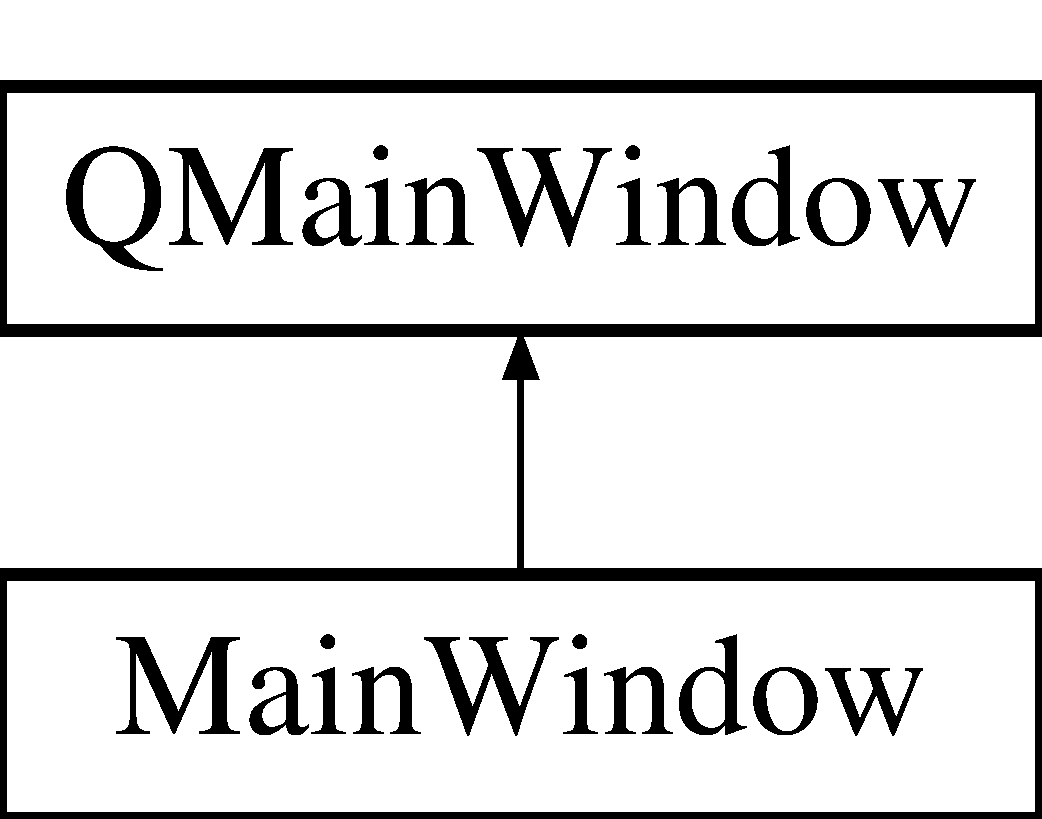
\includegraphics[height=2.000000cm]{class_main_window}
\end{center}
\end{figure}
\subsection*{Public Member Functions}
\begin{DoxyCompactItemize}
\item 
\hyperlink{class_main_window_a8b244be8b7b7db1b08de2a2acb9409db}{Main\-Window} (Q\-Widget $\ast$parent=0)
\item 
bool \hyperlink{class_main_window_adb7dbe0ece2eaa1a92b3ee1da8ae3327}{jugada\-Valida} (int casilla, int valor)
\item 
bool \hyperlink{class_main_window_ab68ff992b159d33b1f80606deabe0361}{jugada\-Correcta} (int casilla)
\item 
void \hyperlink{class_main_window_a18e451ac33947c4e8c058a5266daafbd}{creacion\-Numeros} (int indice, int valor\-Correcto, int col, int fila, int visible)
\item 
void \hyperlink{class_main_window_af0799066013e5dac6614367dc715d3e4}{creacion\-Botones} ()
\item 
void \hyperlink{class_main_window_ade1681f57a1c4cacefd88030c3f70b23}{inicializar\-Timer} ()
\item 
\hyperlink{class_main_window_ae98d00a93bc118200eeef9f9bba1dba7}{$\sim$\-Main\-Window} ()
\end{DoxyCompactItemize}


\subsection{Constructor \& Destructor Documentation}
\hypertarget{class_main_window_a8b244be8b7b7db1b08de2a2acb9409db}{\index{Main\-Window@{Main\-Window}!Main\-Window@{Main\-Window}}
\index{Main\-Window@{Main\-Window}!MainWindow@{Main\-Window}}
\subsubsection[{Main\-Window}]{\setlength{\rightskip}{0pt plus 5cm}Main\-Window\-::\-Main\-Window (
\begin{DoxyParamCaption}
\item[{Q\-Widget $\ast$}]{parent = {\ttfamily 0}}
\end{DoxyParamCaption}
)\hspace{0.3cm}{\ttfamily [explicit]}}}\label{class_main_window_a8b244be8b7b7db1b08de2a2acb9409db}
\hyperlink{class_main_window}{Main\-Window} Constructor de la clase \hyperlink{class_main_window}{Main\-Window} 
\begin{DoxyParams}{Parameters}
{\em parent} & Padre de la clase \\
\hline
\end{DoxyParams}
\hypertarget{class_main_window_ae98d00a93bc118200eeef9f9bba1dba7}{\index{Main\-Window@{Main\-Window}!$\sim$\-Main\-Window@{$\sim$\-Main\-Window}}
\index{$\sim$\-Main\-Window@{$\sim$\-Main\-Window}!MainWindow@{Main\-Window}}
\subsubsection[{$\sim$\-Main\-Window}]{\setlength{\rightskip}{0pt plus 5cm}Main\-Window\-::$\sim$\-Main\-Window (
\begin{DoxyParamCaption}
{}
\end{DoxyParamCaption}
)}}\label{class_main_window_ae98d00a93bc118200eeef9f9bba1dba7}
$\sim$\-Main\-Window Destructor de la clase \hyperlink{class_main_window}{Main\-Window} 

\subsection{Member Function Documentation}
\hypertarget{class_main_window_af0799066013e5dac6614367dc715d3e4}{\index{Main\-Window@{Main\-Window}!creacion\-Botones@{creacion\-Botones}}
\index{creacion\-Botones@{creacion\-Botones}!MainWindow@{Main\-Window}}
\subsubsection[{creacion\-Botones}]{\setlength{\rightskip}{0pt plus 5cm}void Main\-Window\-::creacion\-Botones (
\begin{DoxyParamCaption}
{}
\end{DoxyParamCaption}
)}}\label{class_main_window_af0799066013e5dac6614367dc715d3e4}
creacion\-Botones Crea un tablero de numeros. \hypertarget{class_main_window_a18e451ac33947c4e8c058a5266daafbd}{\index{Main\-Window@{Main\-Window}!creacion\-Numeros@{creacion\-Numeros}}
\index{creacion\-Numeros@{creacion\-Numeros}!MainWindow@{Main\-Window}}
\subsubsection[{creacion\-Numeros}]{\setlength{\rightskip}{0pt plus 5cm}void Main\-Window\-::creacion\-Numeros (
\begin{DoxyParamCaption}
\item[{int}]{indice, }
\item[{int}]{valor\-Correcto, }
\item[{int}]{col, }
\item[{int}]{fila, }
\item[{int}]{visible}
\end{DoxyParamCaption}
)}}\label{class_main_window_a18e451ac33947c4e8c058a5266daafbd}
creacion\-Numeros Crea un numero y lo agrega al tablero. 
\begin{DoxyParams}{Parameters}
{\em indice} & Indice del arreglo numeros que determina la casilla. \\
\hline
{\em valor\-Correcto} & Valor que se asigna en la generacion del tablero. \\
\hline
{\em col} & Columna a la que corresponde el numero. \\
\hline
{\em fila} & Fila a la que corresponde el numero. \\
\hline
{\em visible} & Verdadero si el numero debe mostrarse, falso si la casilla debe mostrarse vacia. \\
\hline
\end{DoxyParams}
\hypertarget{class_main_window_ade1681f57a1c4cacefd88030c3f70b23}{\index{Main\-Window@{Main\-Window}!inicializar\-Timer@{inicializar\-Timer}}
\index{inicializar\-Timer@{inicializar\-Timer}!MainWindow@{Main\-Window}}
\subsubsection[{inicializar\-Timer}]{\setlength{\rightskip}{0pt plus 5cm}void Main\-Window\-::inicializar\-Timer (
\begin{DoxyParamCaption}
{}
\end{DoxyParamCaption}
)}}\label{class_main_window_ade1681f57a1c4cacefd88030c3f70b23}
inicializar\-Timer Inicializa el cronometro. \hypertarget{class_main_window_ab68ff992b159d33b1f80606deabe0361}{\index{Main\-Window@{Main\-Window}!jugada\-Correcta@{jugada\-Correcta}}
\index{jugada\-Correcta@{jugada\-Correcta}!MainWindow@{Main\-Window}}
\subsubsection[{jugada\-Correcta}]{\setlength{\rightskip}{0pt plus 5cm}bool Main\-Window\-::jugada\-Correcta (
\begin{DoxyParamCaption}
\item[{int}]{casilla}
\end{DoxyParamCaption}
)}}\label{class_main_window_ab68ff992b159d33b1f80606deabe0361}
jugada\-Valida Determina si una jugada es correcta. 
\begin{DoxyParams}{Parameters}
{\em casilla} & Indice del arreglo numeros que determina la casilla. \\
\hline
{\em valor} & \hyperlink{class_numero}{Numero} que se esta asignando en la casilla \\
\hline
\end{DoxyParams}
\begin{DoxyReturn}{Returns}
Verdadero si la jugada es correcta, falso si no lo es. 
\end{DoxyReturn}
\hypertarget{class_main_window_adb7dbe0ece2eaa1a92b3ee1da8ae3327}{\index{Main\-Window@{Main\-Window}!jugada\-Valida@{jugada\-Valida}}
\index{jugada\-Valida@{jugada\-Valida}!MainWindow@{Main\-Window}}
\subsubsection[{jugada\-Valida}]{\setlength{\rightskip}{0pt plus 5cm}bool Main\-Window\-::jugada\-Valida (
\begin{DoxyParamCaption}
\item[{int}]{casilla, }
\item[{int}]{valor}
\end{DoxyParamCaption}
)}}\label{class_main_window_adb7dbe0ece2eaa1a92b3ee1da8ae3327}
jugada\-Valida Determina si una jugada es valida 
\begin{DoxyParams}{Parameters}
{\em casilla} & Indice del arreglo numeros que determina la casilla. \\
\hline
{\em valor} & \hyperlink{class_numero}{Numero} que se esta asignando en la casilla \\
\hline
\end{DoxyParams}
\begin{DoxyReturn}{Returns}
Verdadero si la jugada es valida, falso si no lo es. 
\end{DoxyReturn}


The documentation for this class was generated from the following files\-:\begin{DoxyCompactItemize}
\item 
Sudoku/\hyperlink{mainwindow_8h}{mainwindow.\-h}\item 
Sudoku/mainwindow.\-cpp\end{DoxyCompactItemize}

\hypertarget{class_mejores_puntajes}{\section{Mejores\-Puntajes Class Reference}
\label{class_mejores_puntajes}\index{Mejores\-Puntajes@{Mejores\-Puntajes}}
}
Inheritance diagram for Mejores\-Puntajes\-:\begin{figure}[H]
\begin{center}
\leavevmode
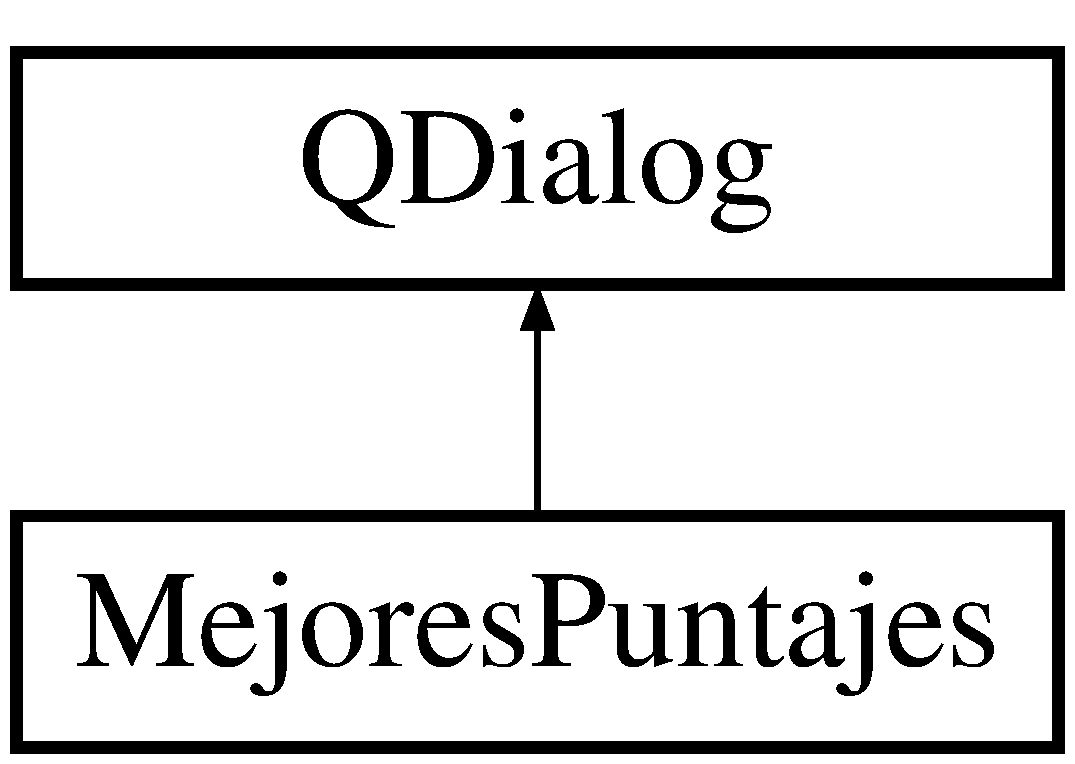
\includegraphics[height=2.000000cm]{class_mejores_puntajes}
\end{center}
\end{figure}
\subsection*{Public Member Functions}
\begin{DoxyCompactItemize}
\item 
\hyperlink{class_mejores_puntajes_a3069d608712a7c7e84df87471b0587bb}{Mejores\-Puntajes} (Q\-Widget $\ast$parent=0)
\item 
\hyperlink{class_mejores_puntajes_a240f173fb76c93d38027261a016244f1}{$\sim$\-Mejores\-Puntajes} ()
\end{DoxyCompactItemize}


\subsection{Constructor \& Destructor Documentation}
\hypertarget{class_mejores_puntajes_a3069d608712a7c7e84df87471b0587bb}{\index{Mejores\-Puntajes@{Mejores\-Puntajes}!Mejores\-Puntajes@{Mejores\-Puntajes}}
\index{Mejores\-Puntajes@{Mejores\-Puntajes}!MejoresPuntajes@{Mejores\-Puntajes}}
\subsubsection[{Mejores\-Puntajes}]{\setlength{\rightskip}{0pt plus 5cm}Mejores\-Puntajes\-::\-Mejores\-Puntajes (
\begin{DoxyParamCaption}
\item[{Q\-Widget $\ast$}]{parent = {\ttfamily 0}}
\end{DoxyParamCaption}
)\hspace{0.3cm}{\ttfamily [explicit]}}}\label{class_mejores_puntajes_a3069d608712a7c7e84df87471b0587bb}
\hyperlink{class_mejores_puntajes}{Mejores\-Puntajes} Constructor de la clase Puntajes 
\begin{DoxyParams}{Parameters}
{\em parent} & Padre de la clase \\
\hline
\end{DoxyParams}
\hypertarget{class_mejores_puntajes_a240f173fb76c93d38027261a016244f1}{\index{Mejores\-Puntajes@{Mejores\-Puntajes}!$\sim$\-Mejores\-Puntajes@{$\sim$\-Mejores\-Puntajes}}
\index{$\sim$\-Mejores\-Puntajes@{$\sim$\-Mejores\-Puntajes}!MejoresPuntajes@{Mejores\-Puntajes}}
\subsubsection[{$\sim$\-Mejores\-Puntajes}]{\setlength{\rightskip}{0pt plus 5cm}Mejores\-Puntajes\-::$\sim$\-Mejores\-Puntajes (
\begin{DoxyParamCaption}
{}
\end{DoxyParamCaption}
)}}\label{class_mejores_puntajes_a240f173fb76c93d38027261a016244f1}
$\sim$\-Mejores\-Puntajes Destructor de la clase Puntajes 

The documentation for this class was generated from the following files\-:\begin{DoxyCompactItemize}
\item 
C\-:/\-Users/user/\-Documents/\-Git\-Hub/\-Sudoku/\-Sudoku/Mejores\-Puntajes.\-h\item 
C\-:/\-Users/user/\-Documents/\-Git\-Hub/\-Sudoku/\-Sudoku/Mejores\-Puntajes.\-cpp\end{DoxyCompactItemize}

\hypertarget{class_mejores_tiempos}{\section{Mejores\-Tiempos Class Reference}
\label{class_mejores_tiempos}\index{Mejores\-Tiempos@{Mejores\-Tiempos}}
}
Inheritance diagram for Mejores\-Tiempos\-:\begin{figure}[H]
\begin{center}
\leavevmode
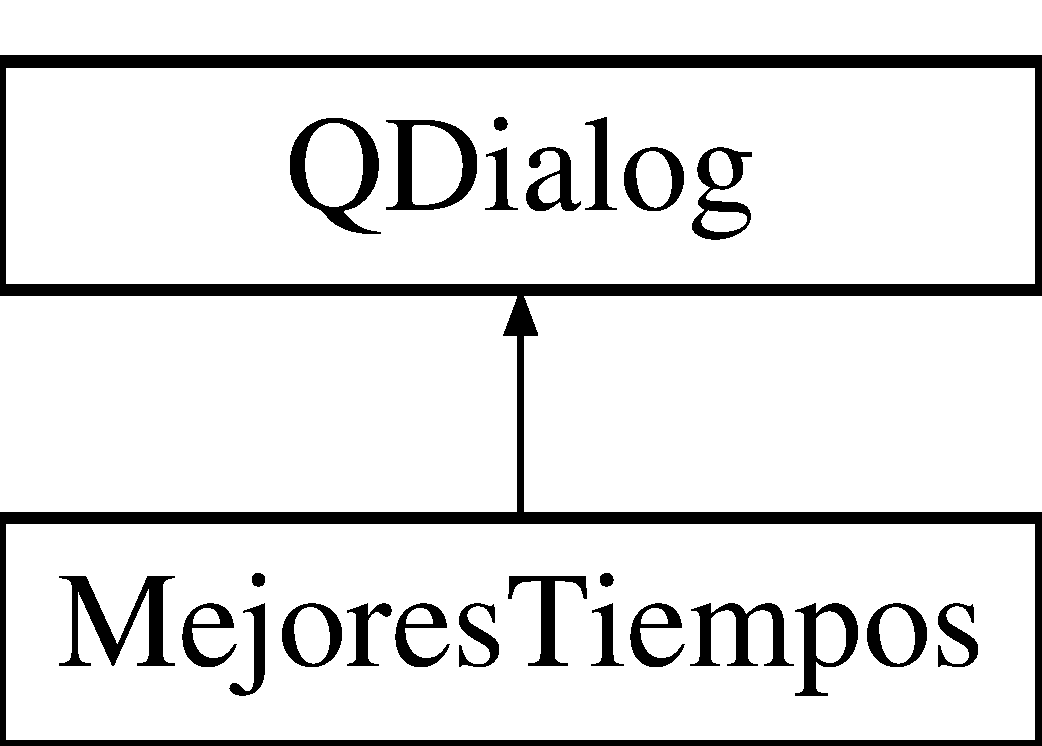
\includegraphics[height=2.000000cm]{class_mejores_tiempos}
\end{center}
\end{figure}
\subsection*{Public Member Functions}
\begin{DoxyCompactItemize}
\item 
\hyperlink{class_mejores_tiempos_a6546ee7792928377484fd761a2e31a01}{Mejores\-Tiempos} (Q\-Widget $\ast$parent=0)
\item 
\hyperlink{class_mejores_tiempos_ac58d13293a8c1905af830cd5e3afdf23}{$\sim$\-Mejores\-Tiempos} ()
\item 
void \hyperlink{class_mejores_tiempos_a7fd2c93312b0df3df68ede23333717c6}{cargar\-Tiempos} ()
\item 
void \hyperlink{class_mejores_tiempos_af32a4917d0f5fbd460f283111690cb5c}{cargar\-Tiempos\-Tabla} ()
\item 
void \hyperlink{class_mejores_tiempos_a23afacd185814cd56a846f9043f223b0}{guardar\-Tiempos} ()
\item 
void \hyperlink{class_mejores_tiempos_a0404cc7b33f26d1d112df3408a7c370c}{ordenar\-Tiempos} (\hyperlink{class_puntaje}{Puntaje} $\ast$puntaje\mbox{[}5\mbox{]})
\end{DoxyCompactItemize}
\subsection*{Public Attributes}
\begin{DoxyCompactItemize}
\item 
\hypertarget{class_mejores_tiempos_af7a18feb7fdea6819c0ac1bf6a22f44c}{\hyperlink{class_puntaje}{Puntaje} $\ast$ {\bfseries list\-Principiante} \mbox{[}5\mbox{]}}\label{class_mejores_tiempos_af7a18feb7fdea6819c0ac1bf6a22f44c}

\item 
\hypertarget{class_mejores_tiempos_a2eab99de3352714326c11d74aad25756}{\hyperlink{class_puntaje}{Puntaje} $\ast$ {\bfseries list\-Intermedio} \mbox{[}5\mbox{]}}\label{class_mejores_tiempos_a2eab99de3352714326c11d74aad25756}

\item 
\hypertarget{class_mejores_tiempos_a4faa9192a0fe4dac0b210e995c4db4bd}{\hyperlink{class_puntaje}{Puntaje} $\ast$ {\bfseries list\-Avanzado} \mbox{[}5\mbox{]}}\label{class_mejores_tiempos_a4faa9192a0fe4dac0b210e995c4db4bd}

\end{DoxyCompactItemize}


\subsection{Constructor \& Destructor Documentation}
\hypertarget{class_mejores_tiempos_a6546ee7792928377484fd761a2e31a01}{\index{Mejores\-Tiempos@{Mejores\-Tiempos}!Mejores\-Tiempos@{Mejores\-Tiempos}}
\index{Mejores\-Tiempos@{Mejores\-Tiempos}!MejoresTiempos@{Mejores\-Tiempos}}
\subsubsection[{Mejores\-Tiempos}]{\setlength{\rightskip}{0pt plus 5cm}Mejores\-Tiempos\-::\-Mejores\-Tiempos (
\begin{DoxyParamCaption}
\item[{Q\-Widget $\ast$}]{parent = {\ttfamily 0}}
\end{DoxyParamCaption}
)\hspace{0.3cm}{\ttfamily [explicit]}}}\label{class_mejores_tiempos_a6546ee7792928377484fd761a2e31a01}
\hyperlink{class_mejores_tiempos}{Mejores\-Tiempos} Constructor de la clase Puntajes 
\begin{DoxyParams}{Parameters}
{\em parent} & Padre de la clase \\
\hline
\end{DoxyParams}
\hypertarget{class_mejores_tiempos_ac58d13293a8c1905af830cd5e3afdf23}{\index{Mejores\-Tiempos@{Mejores\-Tiempos}!$\sim$\-Mejores\-Tiempos@{$\sim$\-Mejores\-Tiempos}}
\index{$\sim$\-Mejores\-Tiempos@{$\sim$\-Mejores\-Tiempos}!MejoresTiempos@{Mejores\-Tiempos}}
\subsubsection[{$\sim$\-Mejores\-Tiempos}]{\setlength{\rightskip}{0pt plus 5cm}Mejores\-Tiempos\-::$\sim$\-Mejores\-Tiempos (
\begin{DoxyParamCaption}
{}
\end{DoxyParamCaption}
)}}\label{class_mejores_tiempos_ac58d13293a8c1905af830cd5e3afdf23}
$\sim$\-Mejores\-Tiempos Destructor de la clase Puntajes 

\subsection{Member Function Documentation}
\hypertarget{class_mejores_tiempos_a7fd2c93312b0df3df68ede23333717c6}{\index{Mejores\-Tiempos@{Mejores\-Tiempos}!cargar\-Tiempos@{cargar\-Tiempos}}
\index{cargar\-Tiempos@{cargar\-Tiempos}!MejoresTiempos@{Mejores\-Tiempos}}
\subsubsection[{cargar\-Tiempos}]{\setlength{\rightskip}{0pt plus 5cm}void Mejores\-Tiempos\-::cargar\-Tiempos (
\begin{DoxyParamCaption}
{}
\end{DoxyParamCaption}
)}}\label{class_mejores_tiempos_a7fd2c93312b0df3df68ede23333717c6}
cargar\-Tiempos Carga los mejores tiempos desde archivo \hypertarget{class_mejores_tiempos_af32a4917d0f5fbd460f283111690cb5c}{\index{Mejores\-Tiempos@{Mejores\-Tiempos}!cargar\-Tiempos\-Tabla@{cargar\-Tiempos\-Tabla}}
\index{cargar\-Tiempos\-Tabla@{cargar\-Tiempos\-Tabla}!MejoresTiempos@{Mejores\-Tiempos}}
\subsubsection[{cargar\-Tiempos\-Tabla}]{\setlength{\rightskip}{0pt plus 5cm}void Mejores\-Tiempos\-::cargar\-Tiempos\-Tabla (
\begin{DoxyParamCaption}
{}
\end{DoxyParamCaption}
)}}\label{class_mejores_tiempos_af32a4917d0f5fbd460f283111690cb5c}
cargar\-Tiempos Carga los mejores tiempos en las tablas \hypertarget{class_mejores_tiempos_a23afacd185814cd56a846f9043f223b0}{\index{Mejores\-Tiempos@{Mejores\-Tiempos}!guardar\-Tiempos@{guardar\-Tiempos}}
\index{guardar\-Tiempos@{guardar\-Tiempos}!MejoresTiempos@{Mejores\-Tiempos}}
\subsubsection[{guardar\-Tiempos}]{\setlength{\rightskip}{0pt plus 5cm}void Mejores\-Tiempos\-::guardar\-Tiempos (
\begin{DoxyParamCaption}
{}
\end{DoxyParamCaption}
)}}\label{class_mejores_tiempos_a23afacd185814cd56a846f9043f223b0}
guardar\-Tiempos Guarda los mejores tiempos en el archivo \hypertarget{class_mejores_tiempos_a0404cc7b33f26d1d112df3408a7c370c}{\index{Mejores\-Tiempos@{Mejores\-Tiempos}!ordenar\-Tiempos@{ordenar\-Tiempos}}
\index{ordenar\-Tiempos@{ordenar\-Tiempos}!MejoresTiempos@{Mejores\-Tiempos}}
\subsubsection[{ordenar\-Tiempos}]{\setlength{\rightskip}{0pt plus 5cm}void Mejores\-Tiempos\-::ordenar\-Tiempos (
\begin{DoxyParamCaption}
\item[{{\bf Puntaje} $\ast$}]{puntaje\mbox{[}5\mbox{]}}
\end{DoxyParamCaption}
)}}\label{class_mejores_tiempos_a0404cc7b33f26d1d112df3408a7c370c}
ordenar\-Tiempos Ordena los tiempos de un arreglo de puntajes 

The documentation for this class was generated from the following files\-:\begin{DoxyCompactItemize}
\item 
C\-:/\-Users/user/\-Documents/\-Git\-Hub/\-Sudoku/\-Sudoku/mejorestiempos.\-h\item 
C\-:/\-Users/user/\-Documents/\-Git\-Hub/\-Sudoku/\-Sudoku/mejorestiempos.\-cpp\end{DoxyCompactItemize}

\hypertarget{class_numero}{\section{Numero Class Reference}
\label{class_numero}\index{Numero@{Numero}}
}
Inheritance diagram for Numero\-:\begin{figure}[H]
\begin{center}
\leavevmode
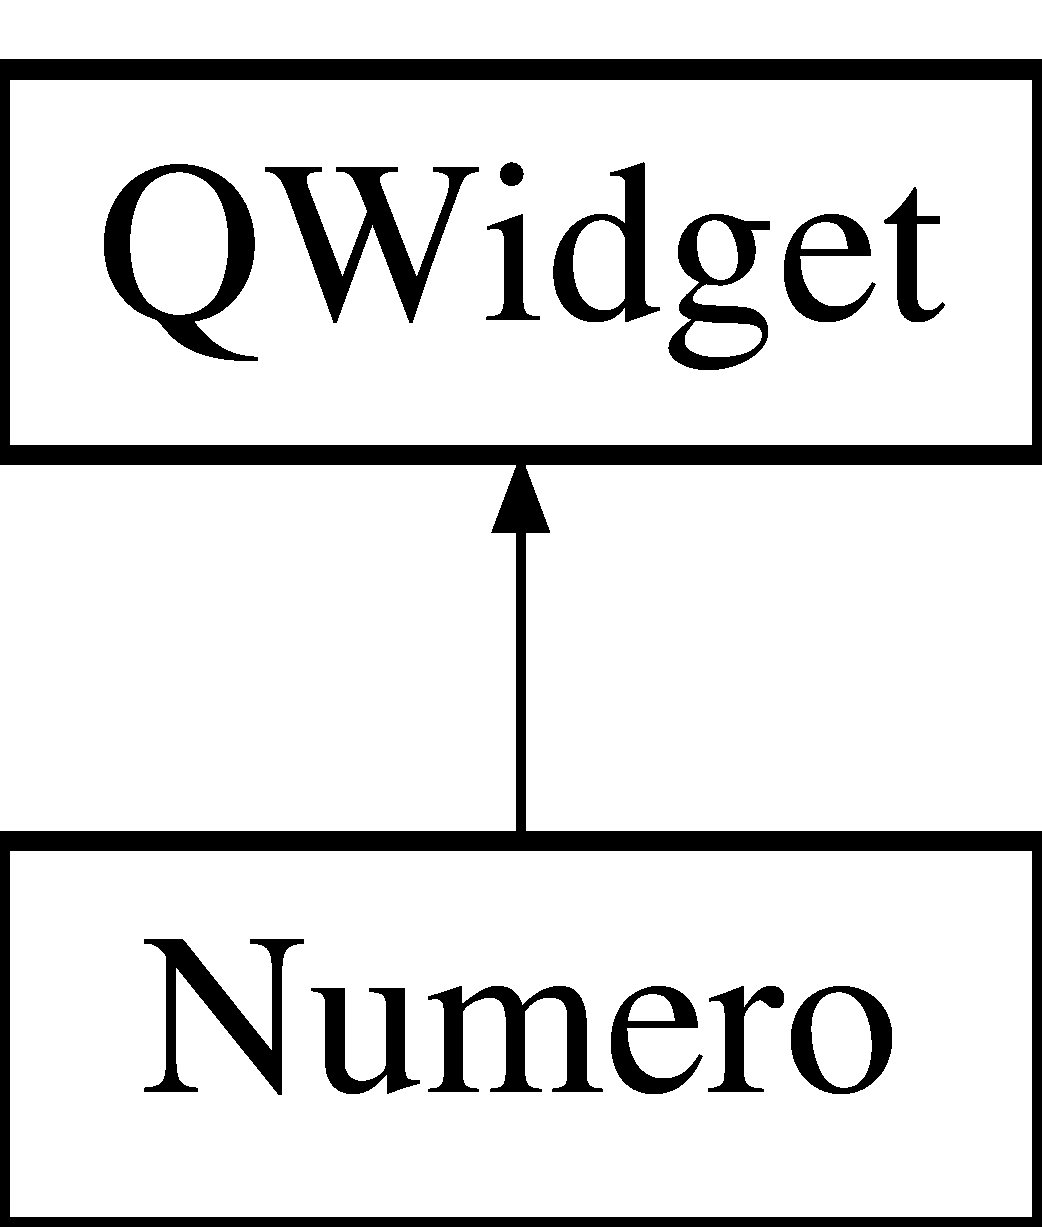
\includegraphics[height=2.000000cm]{class_numero}
\end{center}
\end{figure}
\subsection*{Public Member Functions}
\begin{DoxyCompactItemize}
\item 
\hypertarget{class_numero_a1393437877ace236d969c6dc44ae7ed4}{{\bfseries Numero} (Q\-Object $\ast$parent=0)}\label{class_numero_a1393437877ace236d969c6dc44ae7ed4}

\item 
\hypertarget{class_numero_a390143320c62c9ec5f89d767b8c2ef33}{{\bfseries Numero} (int numero, int columna, int fila, bool visible)}\label{class_numero_a390143320c62c9ec5f89d767b8c2ef33}

\item 
\hypertarget{class_numero_a582df3fe258d20235163d0fbcec712a8}{void {\bfseries set\-Cuadricula} (int fila, int columna)}\label{class_numero_a582df3fe258d20235163d0fbcec712a8}

\item 
\hypertarget{class_numero_a836200e8bd04882bc7ea2f5bc5d7beef}{void {\bfseries set\-Valor} (int valor)}\label{class_numero_a836200e8bd04882bc7ea2f5bc5d7beef}

\item 
\hypertarget{class_numero_ae9002d90ee6ccd3120077c304b85f4fd}{void {\bfseries set\-Valor\-Correcto} (int valor)}\label{class_numero_ae9002d90ee6ccd3120077c304b85f4fd}

\item 
\hypertarget{class_numero_a611e944da6a63813e305287c3f90ad76}{int {\bfseries get\-Fila} (void) const }\label{class_numero_a611e944da6a63813e305287c3f90ad76}

\item 
\hypertarget{class_numero_a4420f97d86be1c1a173405ea37423449}{int {\bfseries get\-Columna} (void) const }\label{class_numero_a4420f97d86be1c1a173405ea37423449}

\item 
\hypertarget{class_numero_ac80a32905356e20d893807572f8b8d4a}{int {\bfseries get\-Cuadricula} (void) const }\label{class_numero_ac80a32905356e20d893807572f8b8d4a}

\item 
\hypertarget{class_numero_ab744d258e626684a3106d39c9cf630b7}{int {\bfseries get\-Valor} (void) const }\label{class_numero_ab744d258e626684a3106d39c9cf630b7}

\item 
\hypertarget{class_numero_a850682763636579e94c90579f74d1308}{int {\bfseries get\-Valor\-Correcto} (void) const }\label{class_numero_a850682763636579e94c90579f74d1308}

\item 
\hypertarget{class_numero_a318e925fff822ed78cd39e382543620c}{void {\bfseries editar\-Boton} (int n)}\label{class_numero_a318e925fff822ed78cd39e382543620c}

\item 
\hypertarget{class_numero_a8a2040801509a6563189dac2a6618372}{void {\bfseries cambiar\-Color\-Boton\-Alerta} ()}\label{class_numero_a8a2040801509a6563189dac2a6618372}

\item 
\hypertarget{class_numero_a1492e35dd63ed7c2a0b6505f755fbf28}{void {\bfseries cambiar\-Color\-Boton\-Pista} ()}\label{class_numero_a1492e35dd63ed7c2a0b6505f755fbf28}

\item 
\hypertarget{class_numero_a8508989f8472de04dd6a4509d1e15814}{void {\bfseries cambiar\-Color\-Boton\-Original} ()}\label{class_numero_a8508989f8472de04dd6a4509d1e15814}

\end{DoxyCompactItemize}
\subsection*{Public Attributes}
\begin{DoxyCompactItemize}
\item 
\hypertarget{class_numero_ae868309035237d255665cc47e11f358e}{Q\-Label $\ast$ {\bfseries label\-Number}}\label{class_numero_ae868309035237d255665cc47e11f358e}

\item 
\hypertarget{class_numero_a05c25be5d0eec99f68ecee2d362a1006}{Q\-Line\-Edit $\ast$ {\bfseries text\-Opciones}}\label{class_numero_a05c25be5d0eec99f68ecee2d362a1006}

\item 
\hypertarget{class_numero_a72aae20a1d5d8722c9da4fa8e97d4efc}{Q\-Push\-Button $\ast$ {\bfseries boton}}\label{class_numero_a72aae20a1d5d8722c9da4fa8e97d4efc}

\item 
\hypertarget{class_numero_a47f3d0b00a7f0c276326be98accb8afa}{Q\-String $\ast$ {\bfseries numero}}\label{class_numero_a47f3d0b00a7f0c276326be98accb8afa}

\end{DoxyCompactItemize}


The documentation for this class was generated from the following files\-:\begin{DoxyCompactItemize}
\item 
Sudoku/\hyperlink{numero_8h}{numero.\-h}\item 
Sudoku/numero.\-cpp\end{DoxyCompactItemize}

\hypertarget{class_posicion}{\section{Posicion Class Reference}
\label{class_posicion}\index{Posicion@{Posicion}}
}
\subsection*{Public Member Functions}
\begin{DoxyCompactItemize}
\item 
\hyperlink{class_posicion_a8d8e3f8286029269c1c19a16c9bd87a5}{Posicion} ()
\item 
\hyperlink{class_posicion_a3a8acc2d5143228949061c773bdb65ec}{Posicion} (int pos, int valor\-\_\-)
\item 
\hyperlink{class_posicion_a192f73b6db15f6c5deeda2445aabeaff}{Posicion} (const \hyperlink{class_posicion}{Posicion} \&other)
\item 
int \hyperlink{class_posicion_a008182c63bfd089f40e793fcb3934570}{Get\-Pos} (void)
\begin{DoxyCompactList}\small\item\em Get\-Pos. \end{DoxyCompactList}\item 
int \hyperlink{class_posicion_afab01c8088eb7f72b28284c5b7b63398}{Get\-Valor} (void)
\begin{DoxyCompactList}\small\item\em Get\-Valor. \end{DoxyCompactList}\end{DoxyCompactItemize}


\subsection{Constructor \& Destructor Documentation}
\hypertarget{class_posicion_a8d8e3f8286029269c1c19a16c9bd87a5}{\index{Posicion@{Posicion}!Posicion@{Posicion}}
\index{Posicion@{Posicion}!Posicion@{Posicion}}
\subsubsection[{Posicion}]{\setlength{\rightskip}{0pt plus 5cm}Posicion\-::\-Posicion (
\begin{DoxyParamCaption}
{}
\end{DoxyParamCaption}
)\hspace{0.3cm}{\ttfamily [inline]}}}\label{class_posicion_a8d8e3f8286029269c1c19a16c9bd87a5}
\hyperlink{class_posicion}{Posicion} Constructor de la clase \hyperlink{class_posicion}{Posicion} 
\begin{DoxyParams}{Parameters}
{\em Constructor} & vacio \\
\hline
\end{DoxyParams}
\hypertarget{class_posicion_a3a8acc2d5143228949061c773bdb65ec}{\index{Posicion@{Posicion}!Posicion@{Posicion}}
\index{Posicion@{Posicion}!Posicion@{Posicion}}
\subsubsection[{Posicion}]{\setlength{\rightskip}{0pt plus 5cm}Posicion\-::\-Posicion (
\begin{DoxyParamCaption}
\item[{int}]{pos, }
\item[{int}]{valor\-\_\-}
\end{DoxyParamCaption}
)\hspace{0.3cm}{\ttfamily [inline]}}}\label{class_posicion_a3a8acc2d5143228949061c773bdb65ec}
\hyperlink{class_posicion}{Posicion} Constructor de la clase \hyperlink{class_posicion}{Posicion} 
\begin{DoxyParams}{Parameters}
{\em pos} & posicion en el tablero \\
\hline
{\em valor} & que tiene esa posicion \\
\hline
\end{DoxyParams}
\hypertarget{class_posicion_a192f73b6db15f6c5deeda2445aabeaff}{\index{Posicion@{Posicion}!Posicion@{Posicion}}
\index{Posicion@{Posicion}!Posicion@{Posicion}}
\subsubsection[{Posicion}]{\setlength{\rightskip}{0pt plus 5cm}Posicion\-::\-Posicion (
\begin{DoxyParamCaption}
\item[{const {\bf Posicion} \&}]{other}
\end{DoxyParamCaption}
)\hspace{0.3cm}{\ttfamily [inline]}}}\label{class_posicion_a192f73b6db15f6c5deeda2445aabeaff}
Posiciones Constructor de la clase Posiciones 
\begin{DoxyParams}{Parameters}
{\em \hyperlink{class_posicion}{Posicion}} & otra clase posicion \\
\hline
\end{DoxyParams}


\subsection{Member Function Documentation}
\hypertarget{class_posicion_a008182c63bfd089f40e793fcb3934570}{\index{Posicion@{Posicion}!Get\-Pos@{Get\-Pos}}
\index{Get\-Pos@{Get\-Pos}!Posicion@{Posicion}}
\subsubsection[{Get\-Pos}]{\setlength{\rightskip}{0pt plus 5cm}int Posicion\-::\-Get\-Pos (
\begin{DoxyParamCaption}
\item[{void}]{}
\end{DoxyParamCaption}
)\hspace{0.3cm}{\ttfamily [inline]}}}\label{class_posicion_a008182c63bfd089f40e793fcb3934570}


Get\-Pos. 

\begin{DoxyReturn}{Returns}
retornar la posicion 
\end{DoxyReturn}
\hypertarget{class_posicion_afab01c8088eb7f72b28284c5b7b63398}{\index{Posicion@{Posicion}!Get\-Valor@{Get\-Valor}}
\index{Get\-Valor@{Get\-Valor}!Posicion@{Posicion}}
\subsubsection[{Get\-Valor}]{\setlength{\rightskip}{0pt plus 5cm}int Posicion\-::\-Get\-Valor (
\begin{DoxyParamCaption}
\item[{void}]{}
\end{DoxyParamCaption}
)\hspace{0.3cm}{\ttfamily [inline]}}}\label{class_posicion_afab01c8088eb7f72b28284c5b7b63398}


Get\-Valor. 

\begin{DoxyReturn}{Returns}
retornar el valor 
\end{DoxyReturn}


The documentation for this class was generated from the following file\-:\begin{DoxyCompactItemize}
\item 
C\-:/\-Users/user/\-Documents/\-Git\-Hub/\-Sudoku/\-Sudoku/\hyperlink{_posicion_8h}{Posicion.\-h}\end{DoxyCompactItemize}

\hypertarget{class_puntaje}{\section{Puntaje Class Reference}
\label{class_puntaje}\index{Puntaje@{Puntaje}}
}
\subsection*{Public Member Functions}
\begin{DoxyCompactItemize}
\item 
\hyperlink{class_puntaje_a3414fcbb7cd0753464c60d03f17b5512}{Puntaje} ()
\item 
\hyperlink{class_puntaje_adf12fc4d5bfa771251cfdb777c747b5d}{Puntaje} (int nivel, Q\-String nombre, Q\-String tiempo, int valor)
\item 
\hypertarget{class_puntaje_adcf607cfc5044a6fbb467979992ef2f4}{void {\bfseries set\-Valores} (int nivel, Q\-String nombre, Q\-String tiempo, int valor)}\label{class_puntaje_adcf607cfc5044a6fbb467979992ef2f4}

\item 
Q\-String \hyperlink{class_puntaje_af098b8673503572df2a530d25712e5e8}{get\-Nombre} (void)
\begin{DoxyCompactList}\small\item\em get\-Nombre \end{DoxyCompactList}\item 
Q\-String \hyperlink{class_puntaje_ac18111ec8685e9fecad20571dc14df3b}{get\-Tiempo} (void)
\begin{DoxyCompactList}\small\item\em get\-Tiempo \end{DoxyCompactList}\item 
int \hyperlink{class_puntaje_aed12d5639a572b00de253b9170fde03f}{get\-Valor} (void)
\begin{DoxyCompactList}\small\item\em get\-Valor \end{DoxyCompactList}\item 
int \hyperlink{class_puntaje_a35b6adcad7bbddf7f38faa0c8de8bd5a}{get\-Nivel} (void)
\begin{DoxyCompactList}\small\item\em get\-Nivel \end{DoxyCompactList}\end{DoxyCompactItemize}


\subsection{Constructor \& Destructor Documentation}
\hypertarget{class_puntaje_a3414fcbb7cd0753464c60d03f17b5512}{\index{Puntaje@{Puntaje}!Puntaje@{Puntaje}}
\index{Puntaje@{Puntaje}!Puntaje@{Puntaje}}
\subsubsection[{Puntaje}]{\setlength{\rightskip}{0pt plus 5cm}Puntaje\-::\-Puntaje (
\begin{DoxyParamCaption}
{}
\end{DoxyParamCaption}
)\hspace{0.3cm}{\ttfamily [inline]}}}\label{class_puntaje_a3414fcbb7cd0753464c60d03f17b5512}
\hyperlink{class_puntaje}{Puntaje} Constructor de la clase \hyperlink{class_puntaje}{Puntaje} 
\begin{DoxyParams}{Parameters}
{\em Constructor} & vacio \\
\hline
\end{DoxyParams}
\hypertarget{class_puntaje_adf12fc4d5bfa771251cfdb777c747b5d}{\index{Puntaje@{Puntaje}!Puntaje@{Puntaje}}
\index{Puntaje@{Puntaje}!Puntaje@{Puntaje}}
\subsubsection[{Puntaje}]{\setlength{\rightskip}{0pt plus 5cm}Puntaje\-::\-Puntaje (
\begin{DoxyParamCaption}
\item[{int}]{nivel, }
\item[{Q\-String}]{nombre, }
\item[{Q\-String}]{tiempo, }
\item[{int}]{valor}
\end{DoxyParamCaption}
)\hspace{0.3cm}{\ttfamily [inline]}}}\label{class_puntaje_adf12fc4d5bfa771251cfdb777c747b5d}
\hyperlink{class_puntaje}{Puntaje} Constructor de la clase \hyperlink{class_puntaje}{Puntaje} 
\begin{DoxyParams}{Parameters}
{\em nombre} & Nombre del jugador \\
\hline
{\em tiempo} & Tiempo que tardo en ganar el juego \\
\hline
{\em nivel} & Nivel del juego \\
\hline
\end{DoxyParams}


\subsection{Member Function Documentation}
\hypertarget{class_puntaje_a35b6adcad7bbddf7f38faa0c8de8bd5a}{\index{Puntaje@{Puntaje}!get\-Nivel@{get\-Nivel}}
\index{get\-Nivel@{get\-Nivel}!Puntaje@{Puntaje}}
\subsubsection[{get\-Nivel}]{\setlength{\rightskip}{0pt plus 5cm}int Puntaje\-::get\-Nivel (
\begin{DoxyParamCaption}
\item[{void}]{}
\end{DoxyParamCaption}
)\hspace{0.3cm}{\ttfamily [inline]}}}\label{class_puntaje_a35b6adcad7bbddf7f38faa0c8de8bd5a}


get\-Nivel 

\begin{DoxyReturn}{Returns}
retornar el nivel 
\end{DoxyReturn}
\hypertarget{class_puntaje_af098b8673503572df2a530d25712e5e8}{\index{Puntaje@{Puntaje}!get\-Nombre@{get\-Nombre}}
\index{get\-Nombre@{get\-Nombre}!Puntaje@{Puntaje}}
\subsubsection[{get\-Nombre}]{\setlength{\rightskip}{0pt plus 5cm}Q\-String Puntaje\-::get\-Nombre (
\begin{DoxyParamCaption}
\item[{void}]{}
\end{DoxyParamCaption}
)\hspace{0.3cm}{\ttfamily [inline]}}}\label{class_puntaje_af098b8673503572df2a530d25712e5e8}


get\-Nombre 

\begin{DoxyReturn}{Returns}
retornar el nombre del jugador 
\end{DoxyReturn}
\hypertarget{class_puntaje_ac18111ec8685e9fecad20571dc14df3b}{\index{Puntaje@{Puntaje}!get\-Tiempo@{get\-Tiempo}}
\index{get\-Tiempo@{get\-Tiempo}!Puntaje@{Puntaje}}
\subsubsection[{get\-Tiempo}]{\setlength{\rightskip}{0pt plus 5cm}Q\-String Puntaje\-::get\-Tiempo (
\begin{DoxyParamCaption}
\item[{void}]{}
\end{DoxyParamCaption}
)\hspace{0.3cm}{\ttfamily [inline]}}}\label{class_puntaje_ac18111ec8685e9fecad20571dc14df3b}


get\-Tiempo 

\begin{DoxyReturn}{Returns}
retornar el tiempo 
\end{DoxyReturn}
\hypertarget{class_puntaje_aed12d5639a572b00de253b9170fde03f}{\index{Puntaje@{Puntaje}!get\-Valor@{get\-Valor}}
\index{get\-Valor@{get\-Valor}!Puntaje@{Puntaje}}
\subsubsection[{get\-Valor}]{\setlength{\rightskip}{0pt plus 5cm}int Puntaje\-::get\-Valor (
\begin{DoxyParamCaption}
\item[{void}]{}
\end{DoxyParamCaption}
)\hspace{0.3cm}{\ttfamily [inline]}}}\label{class_puntaje_aed12d5639a572b00de253b9170fde03f}


get\-Valor 

\begin{DoxyReturn}{Returns}
retornar el valor del tiempo (min$\ast$3600+segundos$\ast$60+milisegundos) 
\end{DoxyReturn}


The documentation for this class was generated from the following file\-:\begin{DoxyCompactItemize}
\item 
C\-:/\-Users/user/\-Documents/\-Git\-Hub/\-Sudoku/\-Sudoku/\hyperlink{puntaje_8h}{puntaje.\-h}\end{DoxyCompactItemize}

\chapter{File Documentation}
\hypertarget{generador_8h}{\section{C\-:/\-Users/user/\-Documents/\-Git\-Hub/\-Sudoku/\-Sudoku/generador.h File Reference}
\label{generador_8h}\index{C\-:/\-Users/user/\-Documents/\-Git\-Hub/\-Sudoku/\-Sudoku/generador.\-h@{C\-:/\-Users/user/\-Documents/\-Git\-Hub/\-Sudoku/\-Sudoku/generador.\-h}}
}


Este archivo contiene la interfaz del generador de Sudokus.  


{\ttfamily \#include $<$stdlib.\-h$>$}\\*
{\ttfamily \#include $<$stack$>$}\\*
{\ttfamily \#include $<$time.\-h$>$}\\*
{\ttfamily \#include $<$Q\-List$>$}\\*
{\ttfamily \#include $<$Q\-Stack.\-h$>$}\\*
{\ttfamily \#include \char`\"{}Posicion.\-h\char`\"{}}\\*
\subsection*{Classes}
\begin{DoxyCompactItemize}
\item 
class \hyperlink{class_generador}{Generador}
\end{DoxyCompactItemize}


\subsection{Detailed Description}
Este archivo contiene la interfaz del generador de Sudokus. \begin{DoxyAuthor}{Author}
Veronica Pozo 

Jose Salas 

Manuel Suarez
\end{DoxyAuthor}
\begin{DoxyDate}{Date}
06/01/2013 
\end{DoxyDate}

\hypertarget{mainwindow_8h}{\section{Sudoku/mainwindow.h File Reference}
\label{mainwindow_8h}\index{Sudoku/mainwindow.\-h@{Sudoku/mainwindow.\-h}}
}


Este archivo contiene la interfaz de la ventana principal.  


{\ttfamily \#include $<$Q\-Main\-Window$>$}\\*
{\ttfamily \#include $<$Q\-Push\-Button$>$}\\*
{\ttfamily \#include $<$Q\-Label$>$}\\*
{\ttfamily \#include $<$Q\-String$>$}\\*
{\ttfamily \#include $<$Q\-Signal\-Mapper$>$}\\*
{\ttfamily \#include $<$Q\-Frame$>$}\\*
{\ttfamily \#include $<$Q\-Widget$>$}\\*
{\ttfamily \#include $<$Q\-Time$>$}\\*
{\ttfamily \#include $<$Q\-Timer$>$}\\*
{\ttfamily \#include $<$Q\-File$>$}\\*
{\ttfamily \#include $<$Q\-Text\-Stream$>$}\\*
{\ttfamily \#include \char`\"{}numero.\-h\char`\"{}}\\*
{\ttfamily \#include \char`\"{}generador.\-h\char`\"{}}\\*
\subsection*{Classes}
\begin{DoxyCompactItemize}
\item 
class \hyperlink{class_main_window}{Main\-Window}
\end{DoxyCompactItemize}


\subsection{Detailed Description}
Este archivo contiene la interfaz de la ventana principal. \begin{DoxyAuthor}{Author}
Veronica Pozo 

Jose Salas 

Manuel Suarez
\end{DoxyAuthor}
\begin{DoxyDate}{Date}
06/01/2013 
\end{DoxyDate}

\hypertarget{numero_8h}{\section{Sudoku/numero.h File Reference}
\label{numero_8h}\index{Sudoku/numero.\-h@{Sudoku/numero.\-h}}
}


Este archivo contiene la interfaz de la clase \hyperlink{class_numero}{Numero}.  


{\ttfamily \#include $<$Q\-Widget$>$}\\*
{\ttfamily \#include $<$Q\-Label$>$}\\*
{\ttfamily \#include $<$Q\-Debug$>$}\\*
{\ttfamily \#include $<$Q\-Line\-Edit$>$}\\*
{\ttfamily \#include $<$Q\-V\-Box\-Layout$>$}\\*
{\ttfamily \#include $<$Q\-Push\-Button$>$}\\*
{\ttfamily \#include $<$Q\-Object$>$}\\*
{\ttfamily \#include $<$Q\-String$>$}\\*
{\ttfamily \#include \char`\"{}Dimensiones.\-h\char`\"{}}\\*
\subsection*{Classes}
\begin{DoxyCompactItemize}
\item 
class \hyperlink{class_numero}{Numero}
\end{DoxyCompactItemize}


\subsection{Detailed Description}
Este archivo contiene la interfaz de la clase \hyperlink{class_numero}{Numero}. \begin{DoxyAuthor}{Author}
Veronica Pozo 

Jose Salas 

Manuel Suarez
\end{DoxyAuthor}
\begin{DoxyDate}{Date}
06/01/2013 
\end{DoxyDate}

\hypertarget{_posicion_8h}{\section{C\-:/\-Users/user/\-Documents/\-Git\-Hub/\-Sudoku/\-Sudoku/\-Posicion.h File Reference}
\label{_posicion_8h}\index{C\-:/\-Users/user/\-Documents/\-Git\-Hub/\-Sudoku/\-Sudoku/\-Posicion.\-h@{C\-:/\-Users/user/\-Documents/\-Git\-Hub/\-Sudoku/\-Sudoku/\-Posicion.\-h}}
}


Este archivo contiene la interfaz de la clase \hyperlink{class_posicion}{Posicion}.  


\subsection*{Classes}
\begin{DoxyCompactItemize}
\item 
class \hyperlink{class_posicion}{Posicion}
\end{DoxyCompactItemize}


\subsection{Detailed Description}
Este archivo contiene la interfaz de la clase \hyperlink{class_posicion}{Posicion}. \begin{DoxyAuthor}{Author}
Veronica Pozo 

Jose Salas 

Manuel Suarez
\end{DoxyAuthor}
\begin{DoxyDate}{Date}
06/01/2013 
\end{DoxyDate}

\hypertarget{puntaje_8h}{\section{C\-:/\-Users/user/\-Documents/\-Git\-Hub/\-Sudoku/\-Sudoku/puntaje.h File Reference}
\label{puntaje_8h}\index{C\-:/\-Users/user/\-Documents/\-Git\-Hub/\-Sudoku/\-Sudoku/puntaje.\-h@{C\-:/\-Users/user/\-Documents/\-Git\-Hub/\-Sudoku/\-Sudoku/puntaje.\-h}}
}


Este archivo contiene la interfaz de la clase \hyperlink{class_puntaje}{Puntaje}.  


{\ttfamily \#include $<$Q\-String$>$}\\*
\subsection*{Classes}
\begin{DoxyCompactItemize}
\item 
class \hyperlink{class_puntaje}{Puntaje}
\end{DoxyCompactItemize}


\subsection{Detailed Description}
Este archivo contiene la interfaz de la clase \hyperlink{class_puntaje}{Puntaje}. \begin{DoxyAuthor}{Author}
Veronica Pozo 

Manuel Suarez
\end{DoxyAuthor}
\begin{DoxyDate}{Date}
07/07/2013 
\end{DoxyDate}

%--- End generated contents ---

% Index
\newpage
\phantomsection
\addcontentsline{toc}{part}{Index}
\printindex

\end{document}
